\documentclass{beamer}
\usepackage{chngpage}
\usepackage{hhline}
\usepackage[utf8]{inputenc}
\usepackage{subcaption}
\usepackage{placeins}
\usepackage{todonotes}
\usepackage{graphics}
\usepackage{graphicx,wrapfig,lipsum}

\usetheme{Copenhagen}

\title{
  Classification of ImageNet\\
  with Convolutional Neural Networks
}
\author{
  Niklas Lindqvist\\
  Thony Price\\
  William Skagerström\\
}

\begin{document}
\maketitle

\begin{frame}
  \frametitle{Agenda}
  \begin{itemize}
    \item Proposal and intention
    \item Implementation
    \item Results \& Discussion
  \end{itemize}
\end{frame}

\section{Proposal and intention}
\subsection{Project proposal}
\begin{frame}
  \frametitle{Project proposal}
  \begin{itemize}
    \item Tiny ImageNet competition
	  \item Implement a CNN
    \item Apply techniques from course to optimize performance of network
  \end{itemize}
\end{frame}

\subsection{Research of the field}
\begin{frame}
  \frametitle{Research of the field}
  \begin{columns}[T]
    \begin{column}{.5\textwidth}
      \begin{block}{}
        \begin{minipage}[c][0.5\textheight][c]{\linewidth}
          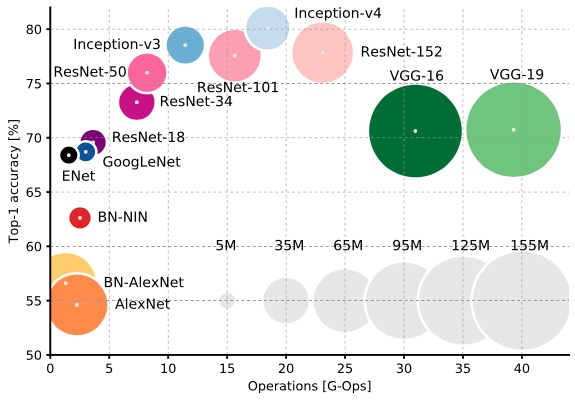
\includegraphics[width=\textwidth]{images/graph_cnns.jpg}
        \end{minipage}
      \end{block}
    \end{column}
    \begin{column}{.5\textwidth}
      \begin{block}{}
        \begin{minipage}[c][0.5\textheight][c]{\linewidth}
          \begin{itemize}
            \item GoogLeNet
            \item RezNet
            \item VGGNet
            \item Stanford's CS231
          \end{itemize}
        \end{minipage}
      \end{block}
    \end{column}
  \end{columns}
\end{frame}

\section{Implementation}
\subsection{Stack and Data}
\begin{frame}
  \frametitle{Stack and Data}
  \centering
  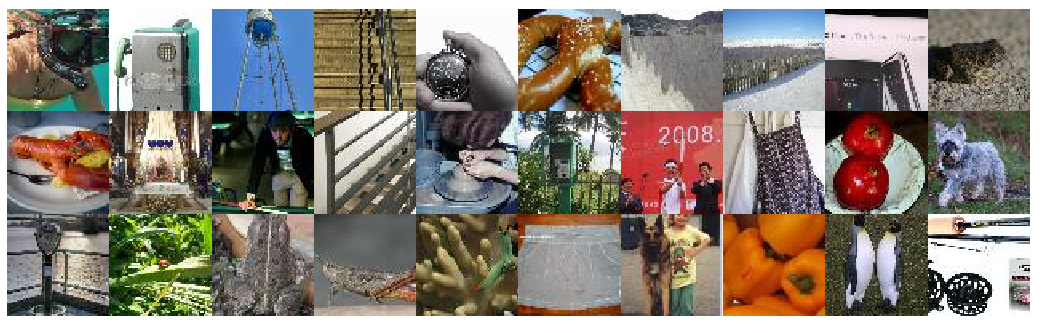
\includegraphics[width=\textwidth]{images/samples.png}
  \vspace{0.05\textheight}
  
\includegraphics[width=\textwidth]{images/logosPNG.png}
\end{frame}

\subsection{CNN configurations}
\begin{frame}
  \frametitle{CNN configurations}
  \medskip

\begin{table}[htbp]
\begin{center}
\scalebox{0.6}{
\begin{tabular}{|c|c|c|c|}

  \hline
  \multicolumn{4}{|c|}{ConvNet Configuration} \\
  \hline

  A & B & C & D
  \\\hline

  SGD, RUI & Adam, RUI, BN &  Adam, RUI, Dropout & Adam, HEI, Dropout, BN
  \\\hhline{|=|=|=|=|}

  \multicolumn{4}{|c|}{input ($64\times64\times3\;RGB\;image$)}
  \\\hline

  conv-32, 2x2, ReLu & conv-32, 2x2, ReLu, BN & conv-32, 2x2, ReLu & conv-32, 2x2, ReLu, BN \\
  conv-32, 2x1, ReLu & conv-32, 2x1, ReLu, BN & conv-32, 2x1, ReLu & conv-32, 2x1, ReLu, BN \\
  conv-32, 1x2, ReLu & conv-32, 1x2, ReLu, BN & conv-32, 1x2, ReLu & conv-32, 1x2, ReLu, BN \\
  \hline
  MaxPooling, 2x2    & MaxPooling, 2x2    & MaxPooling, 2x2    & MaxPooling, 2x2 \\
  \hline
  conv-48, 2x2, ReLu & conv-48, 2x2, ReLu, BN & conv-48, 2x2, ReLu & conv-48, 2x2, ReLu, BN \\
  conv-48, 2x2, ReLu & conv-48, 2x2, ReLu, BN & conv-48, 2x2, ReLu & conv-48, 2x2, ReLu, BN \\
  conv-48, 2x2, ReLu & conv-48, 2x2, ReLu, BN & conv-48, 2x2, ReLu & conv-48, 2x2, ReLu, BN \\
  \hline
  MaxPooling, 2x2    & MaxPooling, 2x2    & MaxPooling, 2x2    & MaxPooling, 2x2 \\
  \hline
  conv-80, 2x2, ReLu & conv-80, 2x2, ReLu, BN & conv-80, 2x2, ReLu & conv-80, 2x2, ReLu, BN \\
  conv-80, 2x2, ReLu & conv-80, 2x2, ReLu, BN & conv-80, 2x2, ReLu & conv-80, 2x2, ReLu, BN \\
  conv-80, 2x2, ReLu & conv-80, 2x2, ReLu, BN & conv-80, 2x2, ReLu & conv-80, 2x2, ReLu, BN \\
  \hline
  MaxPooling, 2x2    & MaxPooling, 2x2        & MaxPooling, 2x2    & MaxPooling, 2x2 \\
  \hline
  FC-2048, ReLu      & FC-2048, ReLu, BN      & FC-2048, ReLu      & FC-2048, ReLu, BN
  \\\hline
  FC-200, SoftMax    & FC-200, SoftMax        & Dropout 0.3        & Dropout 0.3   \\
  \hline
                    &                         & FC-200, SoftMax    & FC-200, SoftMax \\
  \hline
  \end{tabular}
  }
% \caption[]
% {\small
%   Configuration of the four different CNNs tested initially. They differ in terms of solver (SGD/Adam), batch normalization (BN), Dropout and initializer (Random Unit Initialization/He Initialization).
% }
\label{table:3_configurations}
\end{center}
\end{table}

\end{frame}

\section{Results}
\subsection{Initial results}
\begin{frame}
  \centering
  We initialised a run on Google Cloud and the results showed...\pause
  \vspace{0.02\textheight}
  
\includegraphics[width=0.7\textwidth]{images/overfitting.jpeg}
\end{frame}

\subsection{Overfitting...}
\begin{frame}
  \frametitle{Loss plots}
  \centering
  \begin{figure}[!h]
  \centering
  \begin{adjustwidth}{-.4in}{-.4in}
    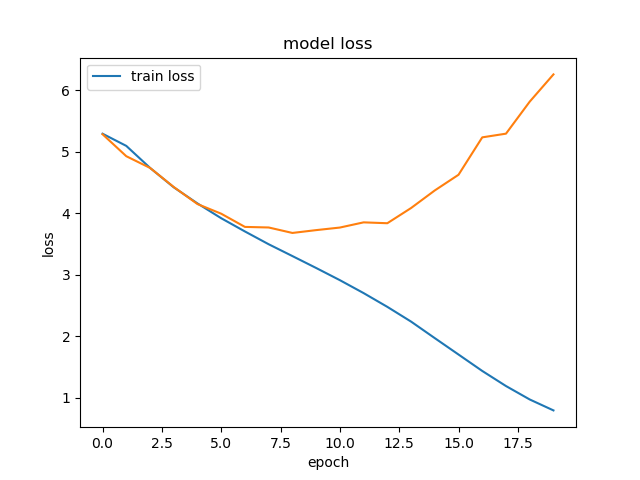
\includegraphics[width=0.4\textwidth]{images/run1_loss_a.png}
    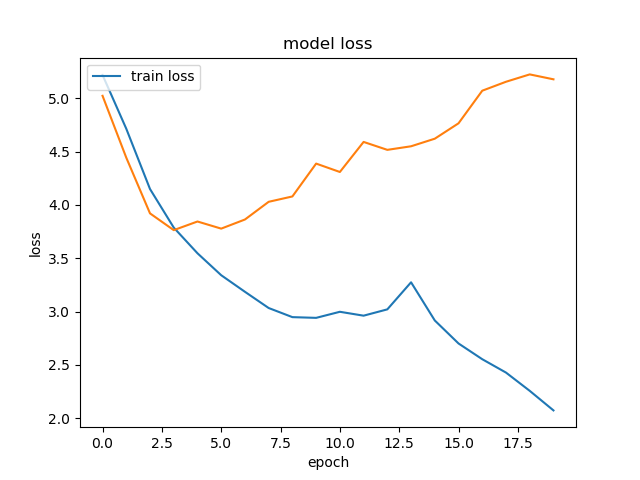
\includegraphics[width=0.4\textwidth]{images/run1_loss_b.png}
    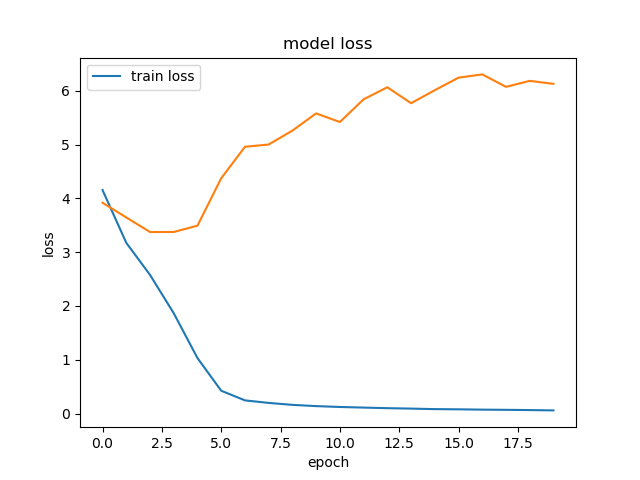
\includegraphics[width=0.4\textwidth]{images/run1_loss_c.png}
  \end{adjustwidth}
  \end{figure}
  (A) \hspace{3.5cm} (B) \hspace{3.5cm} (C)
\end{frame}

\begin{frame}
  \centering
  Network variant D and accuracies
  \begin{figure}[!h]
    \centering
    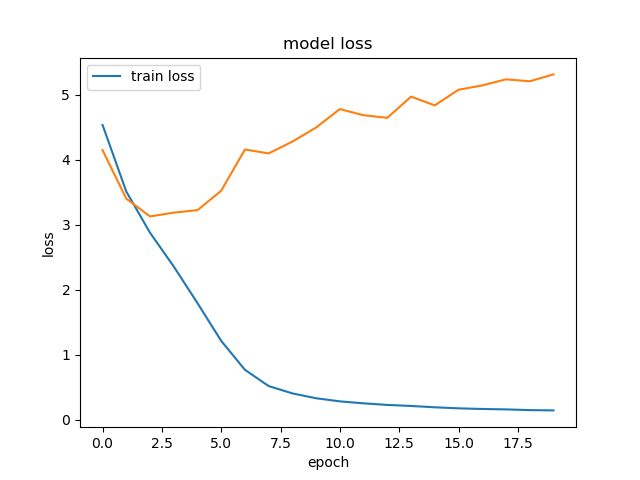
\includegraphics[width=0.5\textwidth]{images/run1_loss_d.png}
  \end{figure}
  

\begin{table}[htbp]
\begin{center}
\begin{tabular}{|l|l|l|l|}
\hline
\textbf{Model} & \textbf{Top-1 val} & \textbf{Top-5 val}  \\
\hline
          A: SGD, RUI                &   17\%  		  &  37\% \\
          B: Adam, RUI, BN           &   22\%  		  &  45\% \\
          C: Adam, RUI, Dropout      &   6\%      	&  20\% \\
          D: Adam, HEI, Dropout, BN  &   29\%  	    &  55\% \\

\hline
\end{tabular}
% \caption[]
% {\small
% Accuracy of models.
% }
\label{table:accuracy}
\end{center}
\end{table}

\end{frame}

\subsection{Prevent overfitting}
\begin{frame}
  \frametitle{Prevent overfitting}
  To battle this we applied
  \begin{itemize}
    \item Batch normalization (All layers)
    \item Dropout (Dense layers)
    \item L2 regularization (X layers)
  \end{itemize}
  And started tinkering with these variables
\end{frame}




\end{document}

%\centering
%Network variant A (left) and B(right)
%\begin{figure}[!h]
%\centering
%\makebox[\textwidth]{
%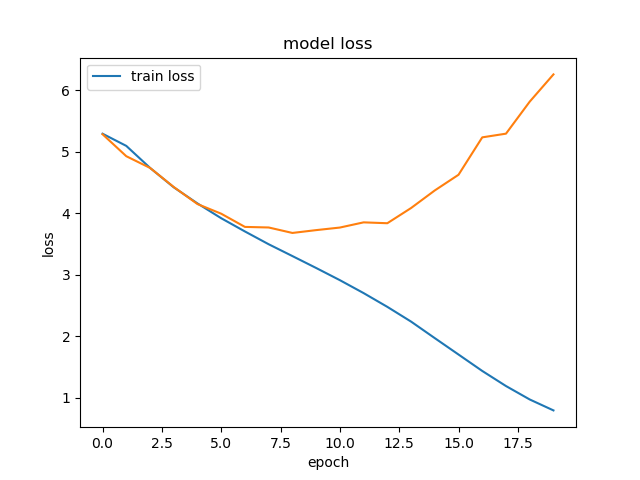
\includegraphics[width=0.3\textwidth]{images/run1_loss_a.png}
%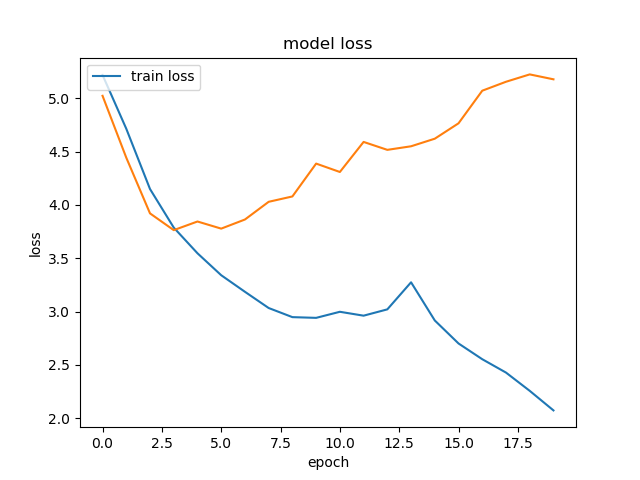
\includegraphics[width=0.3\textwidth]{images/run1_loss_b.png}
%}
%\end{figure}
